\chapter{Эксперимент 5: Исследование конфликтов в кеш-памяти}

\section{Цель эксперимента}
Исследовать влияния конфликтов кэш-памяти на эффективность вычислений.

\section{Описание проблемы}
Наборно-ассоциативная кэш-память состоит из линеек данных, организованных в несколько независимых банков. Выбор банка для каждой порции кэшируемых данных выполняется по ассоциативному принципу, т.е. из условия улучшения представительности выборки, в то время как целевая линейка в каждом из банков жестко определяется по младшей части физического адреса. Совокупность таких линеек всех банков принято называть набором. Таким образом, попытка читать данные из оперативной памяти с шагом, кратным размеру банка, приводит к их помещению в один и тот же набор. Если же количество запросов превосходит степень ассоциативности кэш-памяти, т.е. количество банков или количество линеек в наборе, то наблюдается постоянное вытеснение данных из кэш-памяти, причем  больший ее объем  остается незадействованным.  

\section{Суть эксперимента}
Для определения степени влияния конфликтов в кэш-памяти на эффективность вычислений используется профилировка двух процедур чтения и обработки данных. Первая процедура построена таким образом, что чтение данных выполняется с шагом, кратным размеру банка. Это порождает постоянные конфликты в кэш-памяти. Вторая процедура оптимизирует размещение данных в кэш с помощью задания смещения востребованных данных на некоторый шаг, достаточный для выбора другого набора. Этот шаг соответствует размеру линейки. 

\section{Условия эксперимента}
\begin{enumerate}
    \item Единицы измерения по Ох - Смещение от начала блока;
    \item Единицы измерения по Оу - Такты;
    \item Размер банка кэш-памяти: \textbf{256};
    \item Размер линейки кэш-памяти: \textbf{128};
    \item Количество читаемых линеек: \textbf{512};
\end{enumerate}

\section{Результаты эксперимента}
\begin{figure}[ht!]
    \centering
    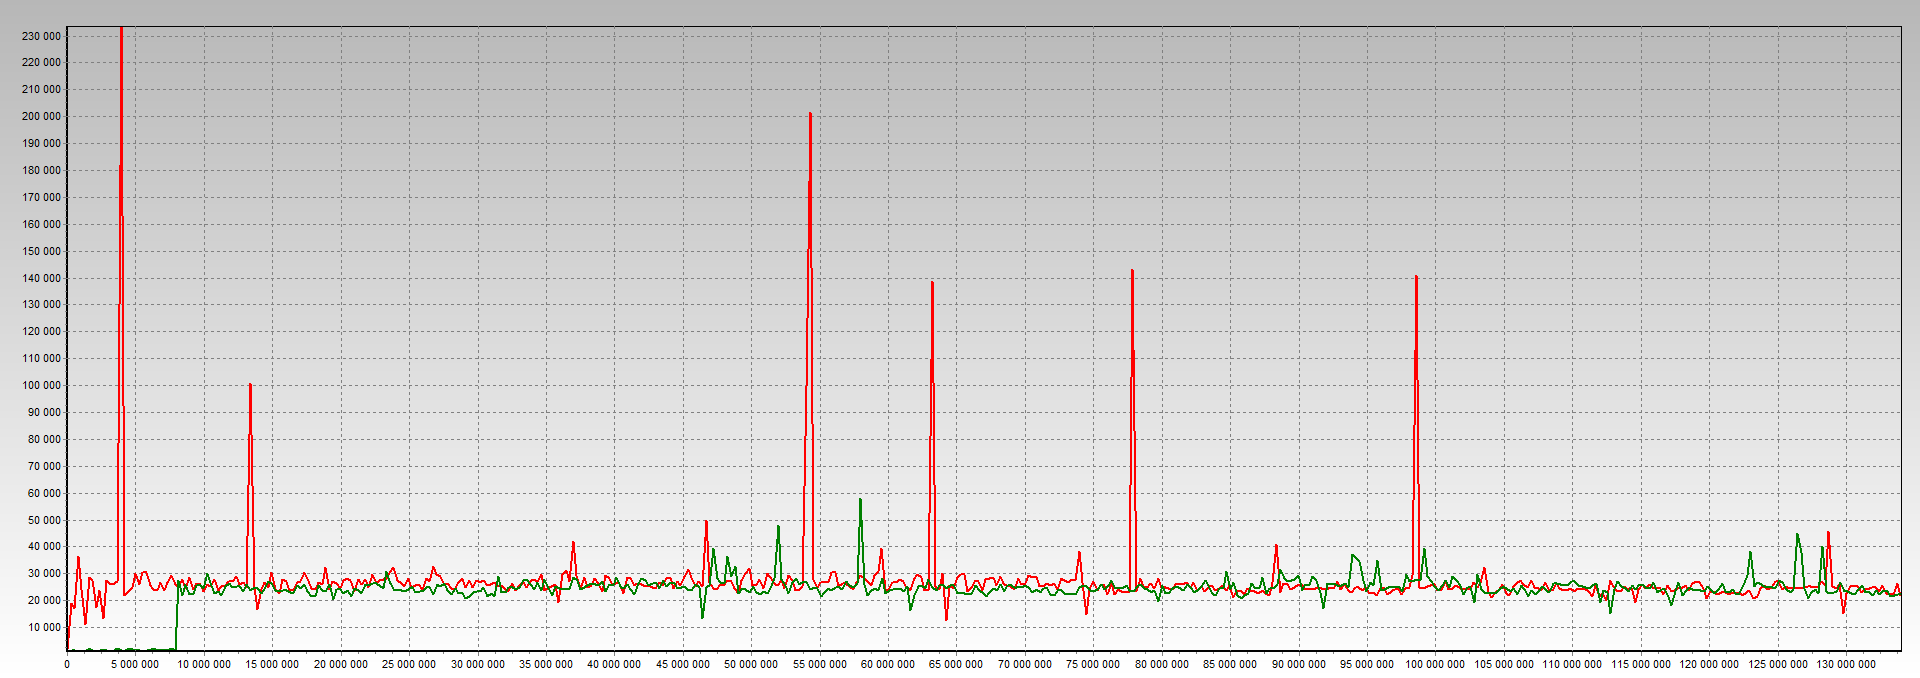
\includegraphics[width=170mm]{./img/task_05.png}
    \caption{Эксперимент 5: Исследование конфликтов в кеш-памяти}
\end{figure}

\begin{figure}[ht!]
    \centering
    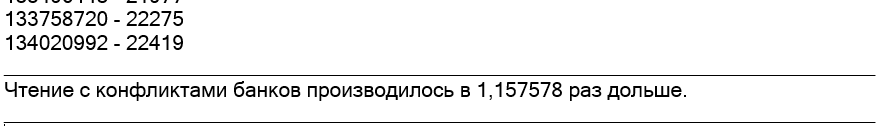
\includegraphics[width=100mm]{./img/res_05.png}
    \caption{Эксперимент 5: Результаты\label{res_05}}
\end{figure}

Как видно на рисунке \ref{res_05}, чтение с конфликтами банков производилось в 1,157578 раз дольше.

\section{Вывод}
Можно сделать вывод, что при использовании кэш-памяти работа процессора ускоряется.